%!TEX root = ../Thesis.tex
\section{Machine Learning in 4D Seismic Time-Shift Extraction}

This final chapter consists of the submitted journal paper \citetitle{dramsch20193dwarping}. This paper presents a novel 3D warping technique for the estimation of 4D seismic time-shifts.

4D seismic time shift extraction is often done in 1D, due to time constraints and often sub-par performance of 3D algorithms. This chapter explores and summarizes conventional 3D warping methods and machine learning approaches. Many of these algorithms rely on classical cross-correlational or optical flow approaches. These approaches suffer from the same limitations in \acl{ml} systems just like conventional algorithms. In this chapter I apply the medical Voxelmorph algorithm to match 4D seismic data.

The algorithm is trained in an unsupervised, or rather self-supervised way to avoid the bias from time shifts that were extracted from another method. The main assumption in the Voxelmorph image alignment depends on diffeomorphic warp velocity fields. The diffeomorphic assumption transfer well to the geological reality that the the mathematical topology stays constant, resulting in reflectors neither crossing nor generating loops. 

\begin{figure}
    \centering
    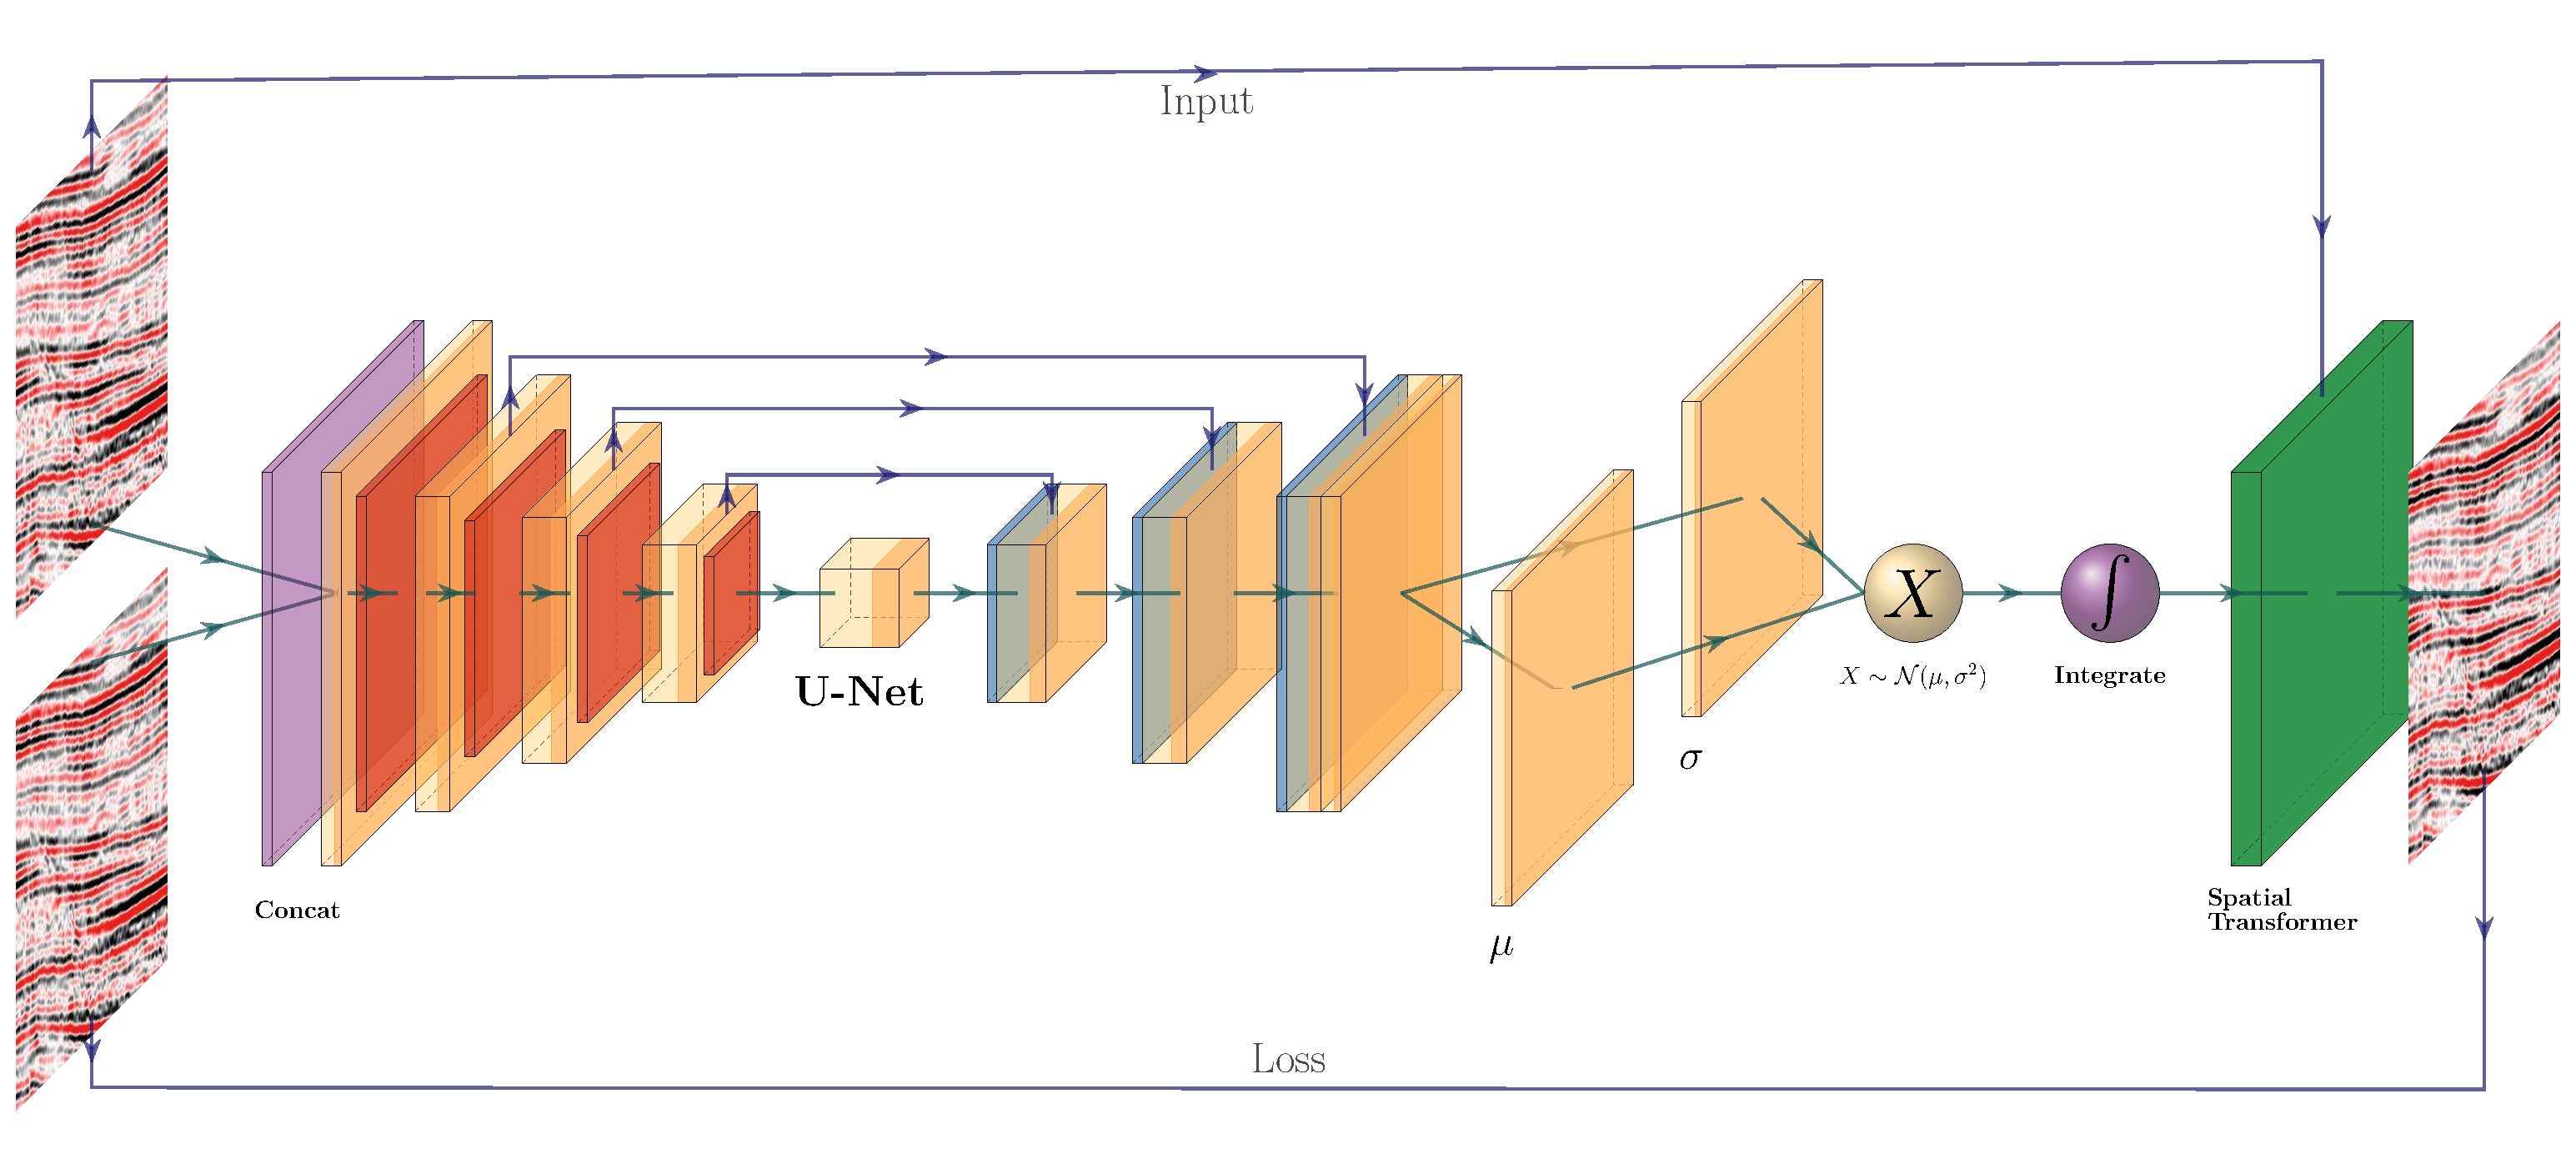
\includegraphics[width=\textwidth]{figures/Voxelmorph.pdf}
    \caption{Voxelmorph Architecture}
    \label{fig:voxelmorph}
\end{figure}
\todo{Extend Description}

The architecture in the network uses the U-Net architecture to input two 3D seismic volumes and extract a static warp velocity field, shown in \cref{fig:voxelmorph}. The static velocity field is extracted as a Gaussian distribution to measure the co-variance and provide uncertainty value of the three-dimensional warp field. The neural network itself does not warp the seismic data, to increase transparency of the process. The architecture following the U-net samples the extracted velocity distribution and integrates this value to obtain the diffeomorphic flow. These values are passed to a dense 3D warping mechanism to enable the unsupervised training. The losses involved are a \acf{kl} on the stationary velocity field and \ac{mse} on the difference between that warped monitor volume and the base volume.

In the paper we present the modified self-supervised \acl{nn} system and test the results on the training data itself and two generalization test sets. The first test set is on the same field but recorded at different times to the training set, ensuring a similar underlying geology, whereas, the second test set is taken from an adjacent field, recorded at different times, testing the full transfer of the trained network. We go on to test the original Voxelmorph architecture, which uses upsampled velocity fields and evaluate the results against our modified architecture, which uses the full flow field. Overall, this technique introduces a generalizable \acl{dl} approach to extract 3D time-shifts with uncertainty measures from raw stacked 4D seismic data.